\documentclass[a4paper]{article}
\usepackage{amsmath}
\usepackage{amssymb}
\usepackage{geometry}
\usepackage{enumerate}
\usepackage{natbib}
\usepackage{float}%稳定图片位置
\usepackage{graphicx,subfig}%画图
\usepackage{caption}
\usepackage[english]{babel}
\usepackage{indentfirst}%缩进
\usepackage{enumerate}%加序号
\usepackage{multirow}%合并行
\usepackage{hyperref}
\newcommand{\reals}{{\mathbb{R}}}
\hypersetup{hypertex=true, colorlinks=true, linkcolor=black, anchorcolor=black, citecolor=black}
\title{\Large \textbf{VG441 Problem Set 1}\\
\author{\textbf{Pan, Chongdan ID:516370910121}\\
}
}
\begin{document}
\maketitle
\section{Problem 1}
\quad
\\$\theta^TX^TX\theta=(X\theta)^T(X\theta)=(X\theta)^2$
\\Assume $X\in\reals^{m\times n},\theta\in\reals^{n\times1}$ then $=(X\theta)^2=\sum_{i=1}^m(\sum_{j=1}^nx_{ij}\theta_j)^2$
\\$\frac{\mathrm{d}\theta^TX^TX\theta^2}{\mathrm{d}\theta}=\frac{\mathrm{d}(X\theta)^2}{\mathrm{d}\theta}=\left[\begin{array}{c}   
    \frac{\partial (X\theta)^2}{\partial \theta_j}\\ 
    \vdots\\  
    \frac{\partial (X\theta)^2}{\partial \theta_n}\\  
  \end{array}\right]
  =\left[\begin{array}{c}   
    2\sum_{i=1}^m(\sum_{j=1}^nx_{ij}x_{i1}\theta_j)\\ 
    \vdots\\  
    2\sum_{i=1}^m(\sum_{j=1}^nx_{ij}x_{in}\theta_j)\\  
  \end{array}\right]$
\\$2X^TX\theta=2\left[\begin{array}{ccc}   
    \sum_{i=1}^mx_{i1}x_{i1} &\cdots & \sum_{i=1}^mx_{i1}x_{in}\\ 
    \vdots&\vdots &\vdots\\  
    \sum_{i=1}^mx_{in}x_{i1} &\cdots & \sum_{i=1}^mx_{in}x_{in}\\  
  \end{array}\right]\left[\begin{array}{c}
    \theta_1\\
    \vdots\\
    \theta_n\\    
  \end{array}\right]=\left[\begin{array}{c}   
    2\sum_{i=1}^m(\sum_{j=1}^nx_{ij}x_{i1}\theta_j)\\ 
    \vdots\\  
    2\sum_{i=1}^m(\sum_{j=1}^nx_{ij}x_{in}\theta_j)\\  
  \end{array}\right]$
\\\\\\Therefore, the derivative of $\theta^TX^TX\theta$ with respect to $\theta$ is $2X^TX\theta$
\section{Problem 2}
\begin{itemize}
    \item The average value for salary is 5875.So before the first iteration:
    \begin{table}[htbp]
        \begin{tabular}{|c|c|c|c|c|c|c|}
        \hline
        Age & Home Owner & Car Owner & Having kids & Salary & F0 & PR0 \\ \hline
        40 & YES & YES & YES & 10000 & 5875 & 4125 \\ \hline
        20 & NO & NO & NO & 500 & 5875 & -5375 \\ \hline
        50 & YES & NO & YES & 8000 & 5875 & 2125 \\ \hline
        30 & YES & NO & NO & 5000 & 5875 & -875 \\ \hline
        \end{tabular}
        \end{table}
    \\The deviance is 5118750.
    \\For \textbf{Home Owner} node: deviance is 12666666.67
    \\For \textbf{CAR Owner} node: deviance is 28500000
    \\For \textbf{Having Kids} node:deviance is 12125000
    \\For \textbf{Age $\leq$ 25} node: deviance is 12666666.67
    \\For \textbf{Age $\leq$ 35} node: deviance is 12125000
    \\For \textbf{Age $\leq$ 45} node: deviance is 45166666
    \\\\So we set \textbf{Having Kids} as the highest node, \textbf{Home Owner} as the left lower node,\textbf{CAR Owner} as the right lower node
    \begin{figure}[H]
        \centering
        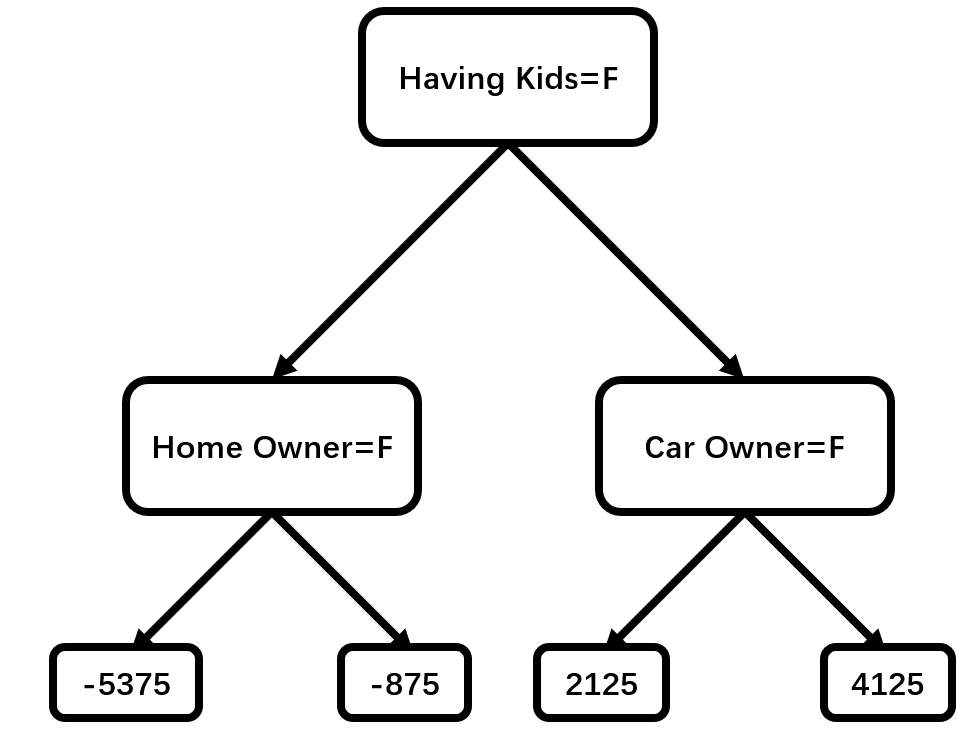
\includegraphics[scale=0.25]{P1.png}
        \caption{First decision tree for GBM}
        \label{P1}
    \end{figure}
    \begin{table}[htbp]
    \begin{tabular}{|c|c|c|c|c|c|c|c|c|c|c|}
        \hline
        Age & Home Owner & Car Owner & Having kids & Salary & F0 & PR0 & F1 & PR1 & F2 & PR2\\ \hline
        40 & YES & YES & YES & 10000 & 5875 & 4125 & 6287.5 & 3712.5 & 6658.75 & 3341.25\\ \hline
        20 & NO & NO & NO & 500 & 5875 & -5375 & 5337.5 & -4837.5 & 4853.75 & -4353.75\\ \hline
        50 & YES & NO & YES & 8000 & 5875 & 2125 & 6087.5 & 1912.5 & 6278.5 & 1721.25\\ \hline
        30 & YES & NO & NO & 5000 & 5875 & -875 & 5787.5 & -787.5 & 5708.75 & -708.75\\ \hline
        \end{tabular}
    \end{table}
    \item The average value for salary is 5875.So before the first iteration:
    \begin{table}[htbp]
        \begin{tabular}{|c|c|c|c|c|c|c|}
        \hline
        Age & Home Owner & Car Owner & Having kids & Salary & F0 & PR0 \\ \hline
        40 & YES & YES & YES & 10000 & 5875 & 4125 \\ \hline
        20 & NO & NO & NO & 500 & 5875 & -5375 \\ \hline
        50 & YES & NO & YES & 8000 & 5875 & 2125 \\ \hline
        30 & YES & NO & NO & 5000 & 5875 & -875 \\ \hline
        \end{tabular}
        \end{table}
        \\SS with $\lambda=1$ is 994050000
        \\For \textbf{Home Owner} node: Gain is 21667968.75
        \\For \textbf{CAR Owner} node: Gain is 12761718.75
        \\For \textbf{Having Kids} node:Gain is 26041666.67
        \\For \textbf{Age $\leq$ 25} node: Gain is 21667968.75
        \\For \textbf{Age $\leq$ 35} node: Gain is 26041666.67
        \\For \textbf{Age $\leq$ 45} node: Gain is 3386718.75
        \\\\So we set \textbf{Having Kids} as the highest node, \textbf{Home Owner} as the left lower node,\textbf{CAR Owner} as the right lower node
        \\The \textbf{Home Owner} node has Gain with $1807292>\gamma$, so it'll remain.
        \\The \textbf{CAR Owner} node has Gain with $-2255208<\gamma$, so it'll be deleted.
        \\After pruning, the XGBoost tree becomes:
        \begin{figure}[H]
            \centering
            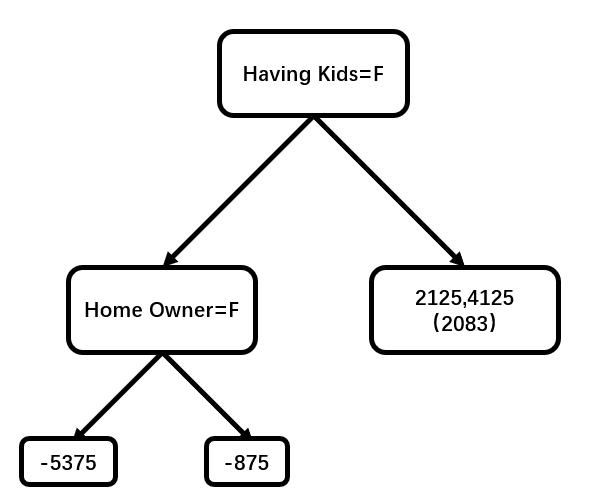
\includegraphics[scale=0.25]{P2.png}
            \caption{First XGBoost Tree}
            \label{P2}
        \end{figure}
        \begin{table}[htbp]
            \begin{tabular}{|c|c|c|c|c|c|c|c|c|c|c|}
                \hline
                Age & Home Owner & Car Owner & Having kids & Salary & F0 & PR0 & F1 & PR1 & F2 & PR2\\ \hline
                40 & YES & YES & YES & 10000 & 5875 & 4125 & 6083.3 & 3916.7 & 6277.75 & 3722.25\\ \hline
                20 & NO & NO & NO & 500 & 5875 & -5375 & 5606.3 & -5106.3 & 5351 & -4851\\ \hline
                50 & YES & NO & YES & 8000 & 5875 & 2125 & 6083.3 & 1916.7 & 6277.75 & 1722.25\\ \hline
                30 & YES & NO & NO & 5000 & 5875 & -875 & 5831.3 & -831.3 & 5790 & -790\\ \hline
                \end{tabular}
            \end{table}
\end{itemize}
\section{Problem 3}
\begin{itemize}
    \item The Linear Regression model leads to $MSE=3.74\times10^9, R^2=0.66$
    \begin{figure}[H]
        \centering
        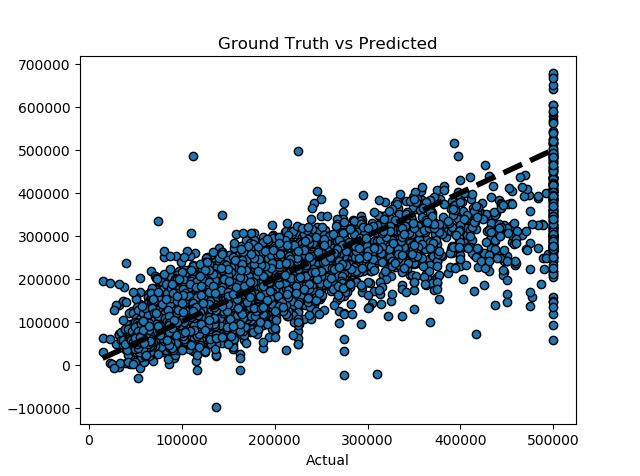
\includegraphics[scale=0.5]{LR.png}
        \caption{Actual Value vs Linear Regression Predicted Value}
        \label{LR}
    \end{figure}
    \item The GBM model leads to $MSE=2.01\times10^9, R^2=0.81$
    \begin{figure}[H]
        \centering
        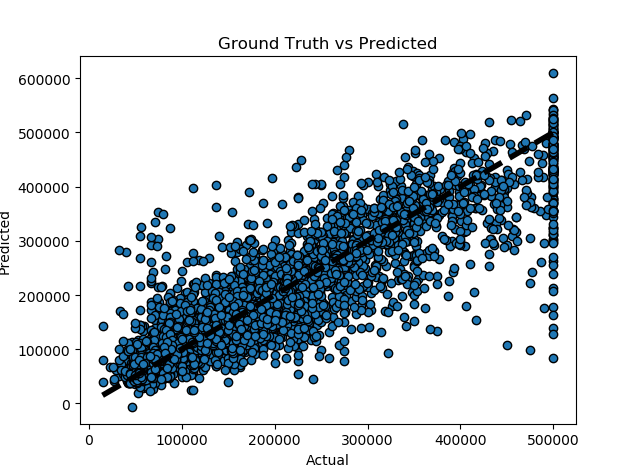
\includegraphics[scale=0.5]{GBM.png}
        \caption{Actual Value vs Gradient Boosting Predicted Value}
        \label{GBM}
    \end{figure}
    \item The XGBoost model leads to $MSE=1.85\times10^9, R^2=0.83$
    \begin{figure}[H]
        \centering
        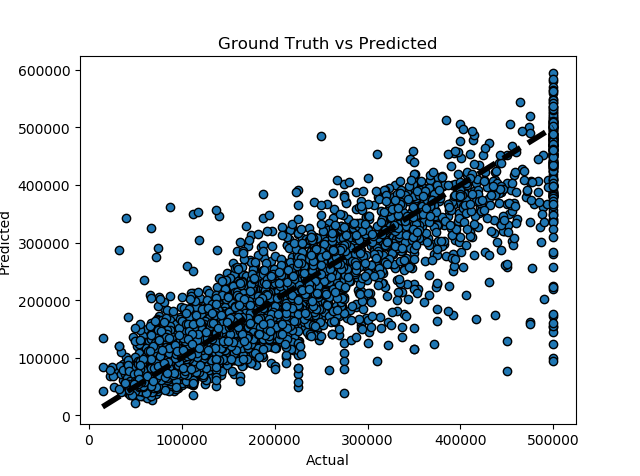
\includegraphics[scale=0.5]{XGBoost.png}
        \caption{Actual Value vs XGBoost Predicted Value}
        \label{XGBoost}
    \end{figure}
\end{itemize}
From the figure, $MSE,R^2$ we get that the XGBoost Model can achieve the best prediction result, and Linear Regression Model's result is worst.
\section*{Python Code}
\begin{verbatim}
import numpy as np
import pandas as pd
import matplotlib.pyplot as plt
from sklearn import linear_model
from sklearn.model_selection import train_test_split
from sklearn.metrics import mean_squared_error, r2_score
from sklearn.model_selection import cross_val_predict

df=pd.DataFrame(pd.read_csv(r"D:\PANDA\Study\VG441\Homework\Problem Set 1\Cal_Housing.csv"))

class_mapping={'NEAR BAY':0, 'INLAND':1}
df['ocean_proximity']=df['ocean_proximity'].map(class_mapping) # 字符串转数字
df=df.dropna(axis=0,how='any',inplace=False) # 删除数据中所有含有nan的行

X=df[['longitude','latitude','housing_median_age','total_rooms','total_bedrooms','population','households','median_income','ocean_proximity']]
Y=df[['median_house_value']]
X_train,X_test,Y_train,Y_test=train_test_split(X, Y, test_size=0.8)
\end{verbatim}
\subsection*{Linear Regression Model}
\begin{verbatim}
model=linear_model.LinearRegression()
\end{verbatim}
\subsection*{GBM Model}
\begin{verbatim}
params = {'n_estimators': 500, 'max_depth': 4, 'min_samples_split': 2, 'learning_rate': 0.05, 'loss': 'ls'}
model = ensemble.GradientBoostingRegressor(**params)
\end{verbatim}
\subsection*{XGBoost Model}
\begin{verbatim}
params = {'n_estimators': 500, "objective":"reg:linear",'colsample_bytree': 0.5,'learning_rate': 0.05,
                'max_depth': 5, 'alpha': 1}
model = xgb.XGBRegressor(**params)
\end{verbatim}
\subsection*{Model Fit}
\begin{verbatim}
model.fit(X_train, Y_train)
model_score = model.score(X_train,Y_train)
Y_predicted = model.predict(X_test)
\end{verbatim}
\subsection*{Result and Visualization}
\begin{verbatim}
print("Mean squared error: %.2f"% mean_squared_error(Y_test, Y_predicted))
print('R2 sq: ',r2_score(Y_test, Y_predicted))
fig, ax = plt.subplots()
ax.scatter(Y_test, Y_predicted, edgecolors=(0, 0, 0))
ax.plot([Y_test.min(), Y_test.max()], [Y_test.min(), Y_test.max()], 'k--', lw=4)
ax.set_xlabel('Actual')
ax.set_ylabel('Predicted')
ax.set_title("Ground Truth vs Predicted")
plt.show()
\end{verbatim}
\end{document}